\documentclass[12pt]{article}

\usepackage{amsmath}
\usepackage{amsfonts}
\usepackage{amssymb}
\usepackage{graphicx}
\usepackage[center]{caption}
\usepackage{mathtools}
\usepackage{lipsum}
\usepackage{stackengine}
\usepackage{fancyhdr}
\usepackage{caption}
\usepackage{tikz}
\usetikzlibrary{shapes.geometric, arrows}
\usepackage{float}
\usepackage[a4paper,left=1in,right=1in,top=1in,bottom=1in,footskip=.25in]{geometry}
\usepackage{etoolbox}
\usepackage[nottoc]{tocbibind}
\usepackage{tabu}
\usepackage{enumitem,kantlipsum}
\usepackage{verbatim}
\usepackage{hyperref}
\begin{document}


\section{Aim}
This test case is for checking the capability of the written Isogeometric analysis code with a linear elastic loading.
\section{Problem description} \label{2DPWLELPD}
\emph{Section 7.1.1 in Documentation}\\
A 2D plate is subjected to mechanical loading as shown in Figure(\ref{XYLoading}). The material used is PZT-PIC151 ceramics.
The movement of bottom edge AB is fixed in y-direction and left edge AC in x-direction. A displacement of 100 nm (1e-4 mm) is given on the right edge BD.
\begin{figure}[H]
	\centering
	\begin{minipage}{.5\textwidth}
		\centering
		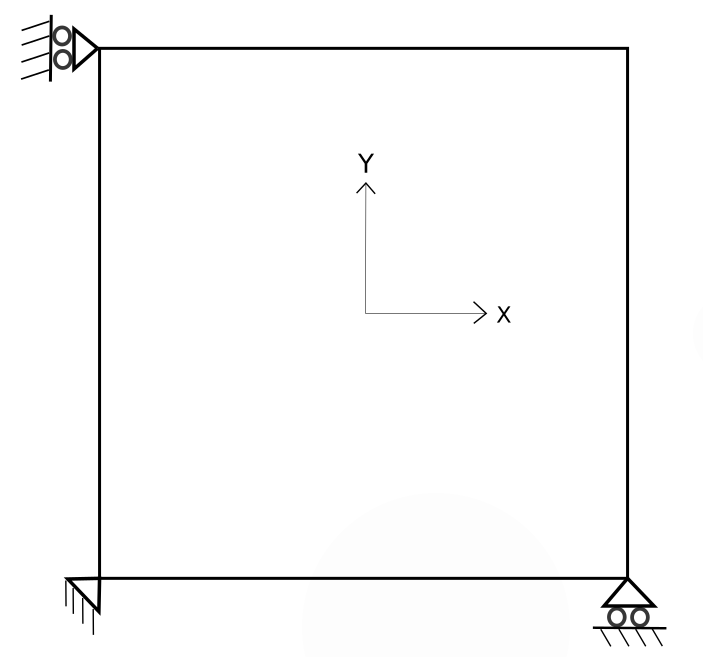
\includegraphics[width=0.8\linewidth]{2DPlate.png}
		\captionof{figure}{2D Plate}
		\label{2Dplate}
	\end{minipage}%
	\begin{minipage}{.5\textwidth}
		\centering
		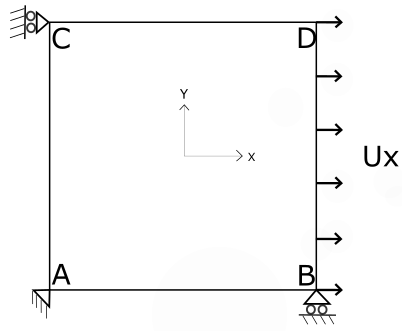
\includegraphics[width=0.9\linewidth]{XYLoading.png}
		\captionof{figure}{2D Plate with loading}
		\label{XYLoading}
	\end{minipage}
\end{figure}
\newpage
\section{How to run the Program}
\begin{enumerate}[leftmargin=*]
	\item The code is written in python and external libraries numpy, matplotlib.pyplot, sys, path from pathlib and math are used.
	\item Please use any environment which will compile python programs
	\item Place all the files in a single folder.
	\item A file named Input.py can be edited to change the dimensions of the plate. User can change Length, Height and Thickness of the plate. \\(The results discussed below are for Length = 10 mm, Height = 10 mm and Thickness = 1 mm)
	\begin{figure}[H]
		\begin{center}
			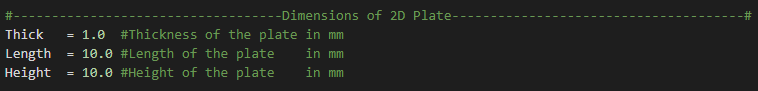
\includegraphics[scale=0.8]{Input.png} 
		\end{center}	
	\end{figure}
	\item Before you run the file, please make sure that the working directory is same as the folder  which
	Consists the Program.
	\item Use command  $>>>$ python Main\_Program.py to run the program.
	\item The contour plots will be saved in the folder \textbf{Results.}
	\item A "log.txt" file is created in the same folder which contains the values of the results plotted.
	 
	
\end{enumerate}
\newpage
\section{Results and discussions} \label{ResultsMech}
Considering the accuracy of the IGA simulation results over FEM results, IGA code generated results can be compared with the Abaqus inbuilt element generated results. An Abaqus plane strain full integration element (\textbf{CPE4}) is used for this purpose.
\\The below figures show the values of displacements (U) and reaction forces (RF ) for both Abaqus and IGA element.\\

\textbf{A similar contour is used for the program generated results and Abaqus results for easy comparison. }\\
Figure(\ref{M1U1}) and Figure(\ref{M1U1_IGA}) show the displacement (U1) values of the single CPE4 element and single IGA element at 100 \% loading in x-direction respectively. \\
\begin{figure}[H]
	\centering
	\begin{minipage}{.5\textwidth}
		\centering
		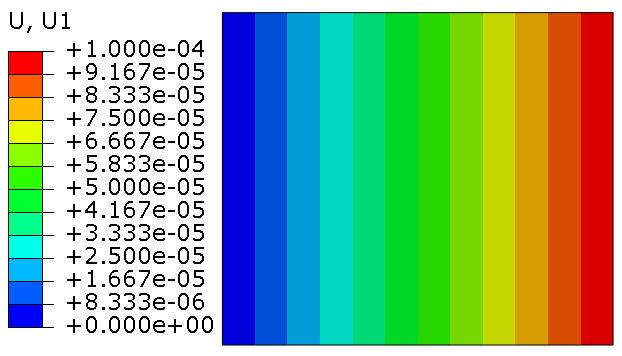
\includegraphics[width=1\linewidth]{M1U1.png}
		\captionof{figure}{CPE4 Element:U1 \\\textbf{Abaqus generated result}}
		\label{M1U1}
	\end{minipage}%
	\begin{minipage}{.55\textwidth}
		\centering
		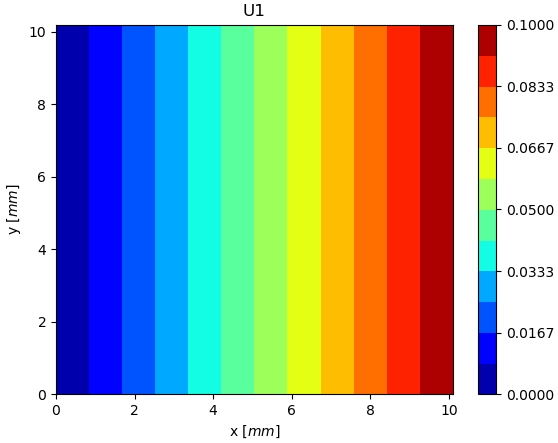
\includegraphics[width=1\linewidth]{M1U1_IGA.png}
		\captionof{figure}{IGA Element:U1 \\ \textbf{Program generated result}}
		\label{M1U1_IGA}
	\end{minipage}
\end{figure}
\begin{comment}
\begin{figure}[H]
\begin{center}
\includegraphics[scale=0.45]{xyz.png} 
\caption{\\CPE4 Element U1}\label{xyz}
\end{center}	
\end{figure}

\begin{figure}[H]
\begin{center}
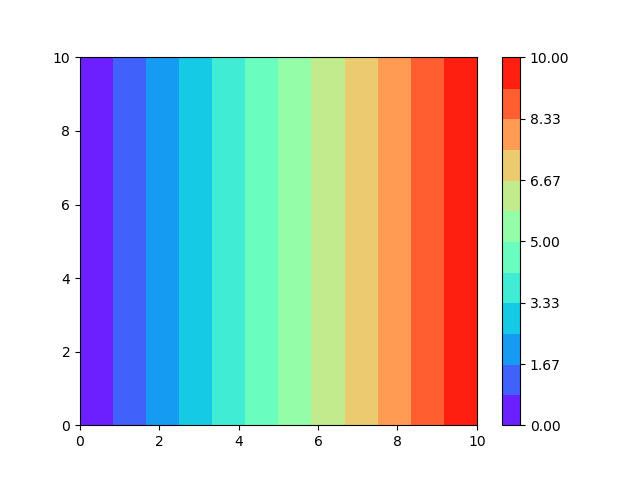
\includegraphics[scale=0.8]{Figure_1.png} 
\caption{\\IGA Element U1}\label{Figure_1}
\end{center}	
\end{figure}
\end{comment}
Figure(\ref{M1U2}) and Figure(\ref{M1U2_IGA}) show the displacement (U2) values of the single CPE4 element and single IGA element at 100 \% loading in y-direction respectively. \\
\begin{figure}[H]
	\centering
	\begin{minipage}{.5\textwidth}
		\centering
		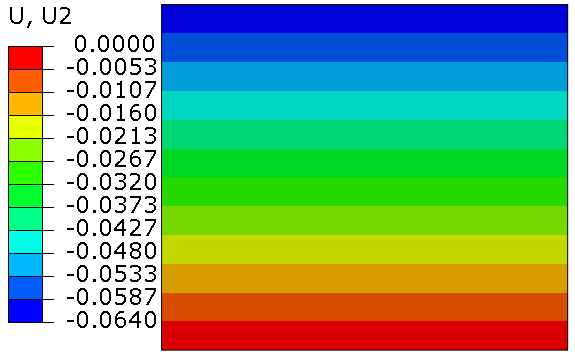
\includegraphics[width=1\linewidth]{M1U2.png}
		\captionof{figure}{CPE4 Element:U2
			\\\textbf{Abaqus generated result}}
		\label{M1U2}
	\end{minipage}%
	\begin{minipage}{.55\textwidth}
		\centering
		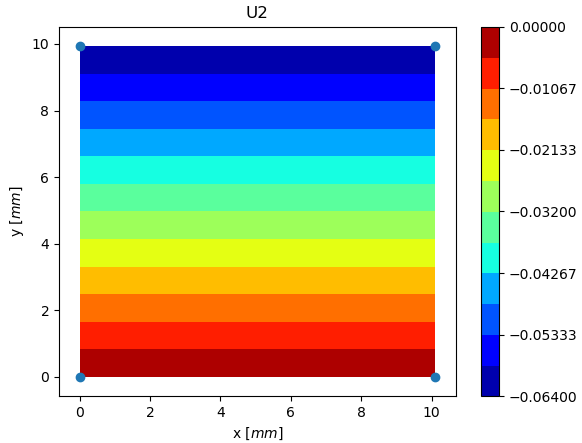
\includegraphics[width=1\linewidth]{M1U2_IGA.png}
		\captionof{figure}{IGA Element:U2\\ \textbf{Program generated result}}
		\label{M1U2_IGA}
	\end{minipage}
\end{figure}



Figure(\ref{M1RF1}) and Figure(\ref{M1RF1_IGA}) show the Reaction force values (RF1) of the single CPE4 element and single IGA element at 100 \% loading in x-direction respectively. \\
\begin{figure}[H]
	\centering
	\begin{minipage}{.5\textwidth}
		\centering
		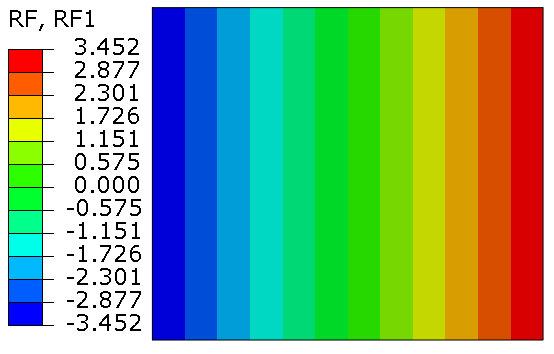
\includegraphics[width=1\linewidth]{M1RF1.png}
		\captionof{figure}{CPE4 Element:RF1
			\\\textbf{Abaqus generated result}}
		\label{M1RF1}
	\end{minipage}%
	\begin{minipage}{.65\textwidth}
		\centering
		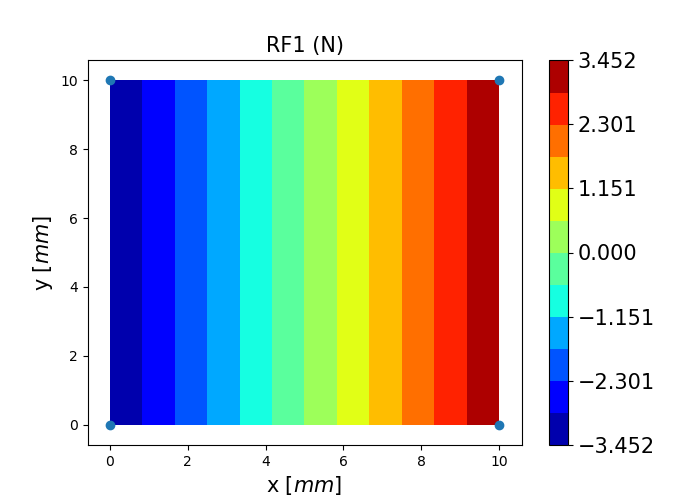
\includegraphics[width=1\linewidth]{M1RF1_IGA.png}
		\captionof{figure}{IGA Element:RF1\\ \textbf{Program generated result}}
		\label{M1RF1_IGA}
	\end{minipage}
\end{figure}

\textbf{Reaction force in the y-direction is not reported since the loading is given only in the x-direction, and for the given fixed BCS, the RF2 is negligible.}  \\


\end{document}